\chapter{Introducción}
\label{ch:introducción}
\section{Definición del problema}

No es una novedad que el crecimiento del \textit{parque móvil}\footnote{\textbf{Parque móvil}: Conjunto total de vehículos registrados y en circulación en una determinada región o país.} y el auge del turismo en las Islas Canarias y sobre todo en Tenerife han provocado que encontrar aparcamiento en prácticamente cualquier lugar resulte cada vez más difícil. En las zonas de alta densidad, como puede ser el \textbf{área metropolitana}, el problema es aún más acentuado, donde tanto residentes como visitantes diariamente sufren un desequilibrio crítico entre oferta y demanda de espacio urbano.

En muchas vías de Tenerife, este problema se manifiesta de forma recurrente en los principales ejes urbanos. Cualquier conductor que transite por la zona que hay entre Santa Cruz de Tenerife y San Cristóbal de La Laguna puede verse atrapado en atascos que, en trayectos de apenas diez kilómetros, generan pérdidas de tiempo significativas y degradan la calidad de vida. Sin embargo, el problema no reside únicamente en la congestión de vías principales como la \textit{(TF-5)}\footnote{\textbf{TF-5}: Es la principal autopista del norte de Tenerife, que conecta Santa Cruz de Tenerife con el área metropolitana y los municipios del norte de la isla.}, sino en la dificultad añadida de encontrar un hueco libre al llegar al destino. De hecho, se estima que hasta un 35\% del tráfico urbano en horas punta está compuesto por vehículos que circulan en bucle buscando estacionamiento~\cite{elpais2025trafico35}, lo que contribuye innecesariamente a la contaminación acústica y a las emisiones de gases de efecto invernadero \textit{(GEI)}\footnote{\textbf{GEI}: Los gases de efecto invernadero son aquellos que contribuyen al calentamiento global al retener el calor en la atmósfera, como el dióxido de carbono (CO$_2$).}.

Moverse por Santa Cruz de Tenerife en hora punta se ha convertido en una prueba de paciencia: el \textit{TomTom Traffic Index}~\cite{tomtom2026} registró en 2025 que los conductores perdieron una media de 52 horas atrapados en el tráfico y un índice de congestión del 34,8\%, lo que equivale a pasar más de dos días enteros al año prácticamente parados en cola. El gran embudo diario llega con  el atardecer, cuando la velocidad cae a unos desesperantes 28 km/h y la congestión alcanza el 55,7\%.

Resulta irónico que, mientras cientos de conductores pierden tiempo y combustible buscando aparcamiento, estas plazas permanezcan vacías durante gran parte del día o incluso durante periodos vacacionales. Este desaprovechamiento de un recurso escaso pone de manifiesto una clara ineficiencia en la gestión del espacio disponible.

Es por ello que, a partir de este gran contraste, nace la motivación de \textbf{Parky} y su principal objetivo: explorar cómo se puede conectar a los propietarios de estas plazas privadas poco usadas con conductores que requieren estacionar su vehículo, facilitando por medio de tecnologías digitales una gestión más inteligente y eficiente de los recursos urbanos existentes.

\medskip
\noindent\textit{Nota terminológica:} a lo largo de la memoria, los términos \textit{arrendador} y \textit{propietario de plaza} se emplean de forma equivalente para referirse al titular del garaje que lo pone en alquiler; del mismo modo, \textit{arrendatario} y \textit{conductor} designan indistintamente a quien realiza la reserva.

\section{Justificación}
\label{sec:justificación}

Parky busca responder a tres factores que convergen en el contexto urbano de 2026: presión normativa, eficiencia económica y madurez tecnológica.

En primer lugar, desde la perspectiva de la \textbf{sostenibilidad y presión regulatoria}, el proyecto responde a la obligatoriedad de implementar Zonas de Bajas Emisiones \textit{(ZBE)} en municipios de más de 50.000 habitantes, como es el caso de Santa Cruz de Tenerife y San Cristóbal de La Laguna. Una parte sustancial del tráfico urbano es generado exclusivamente por la búsqueda de estacionamiento. Facilitar una plataforma \textit{(P2P)}\footnote{\textbf{P2P}: Sistema digital que permite a personas o empresas realizar transacciones directas entre sí, sin la necesidad de intermediarios tradicionales como bancos o grandes empresas.} permite una transición hacia una movilidad más ordenada, reduciendo significativamente las emisiones de gases y el ruido en el centro de las ciudades, alineándose así con los objetivos de las denominadas \textit{Smart Cities}\footnote{\textbf{Smart Cities}: es un entorno urbano que utiliza tecnologías avanzadas, como el Internet de las Cosas (IoT), la inteligencia artificial (IA), el big data y las TIC (Tecnologías de la Información y Comunicación), para mejorar la calidad de vida de sus habitantes, optimizar la gestión de recursos y promover el desarrollo sostenible.}.

En segundo lugar, la \textbf{eficiencia social y económica} del modelo P2P está respaldada por datos: la movilidad compartida registra una tasa de crecimiento anual compuesta (CAGR)\footnote{\textbf{CAGR} (\textit{Compound Annual Growth Rate}): indicador financiero que mide la tasa de crecimiento anual compuesta de una inversión o mercado durante un período determinado, asumiendo la reinversión de los beneficios.} del 14,8\% hasta 2030~\cite{grandviewresearch2022}. \textbf{Parky} permite a los propietarios obtener entre 150 € y 300 € mensuales por una plaza infrautilizada, mientras que ofrece al conductor un ahorro directo de tiempo ya que se dedica de media 24 horas anuales solo a buscar hueco~\cite{inrix2022}.

Por último, la \textbf{viabilidad tecnológica} está respaldada por la madurez del ecosistema disponible. Las APIs de geolocalización, las pasarelas de pago P2P y las bases de datos con seguridad a nivel de fila existen, están documentadas y tienen precios accesibles para un prototipo. El mismo conductor que hoy circula en bucle puede reservar y acceder a una plaza privada en menos de dos minutos desde el móvil.

\section{Estado del arte}
\label{sec:estado-del-arte}

Las plataformas de aparcamiento en 2026 se organizan en cuatro categorías con modelos de negocio y barreras de entrada distintas que se describen a continuación.

\subsection{Aplicaciones de zona regulada}

Las plataformas de zona regulada digitalizan el cobro de tasas de estacionamiento en vía pública mediante contratos con los ayuntamientos. Sin ese convenio, no pueden operar en ninguna ciudad. Esta dependencia institucional define su modelo de expansión y limita su presencia a los municipios que han licitado el servicio.

\textbf{EasyPark}~\cite{easypark2024} opera en más de 4.200 ciudades de 21 países, con más de 6.000 operadores de aparcamiento integrados, resultado de una estrategia de adquisiciones de otras plataformas de este mercado. La filial española, con sede en Barcelona, gestiona la zona regulada en más de 130 ciudades de la península actualmente ~\cite{lavanguardia2024easypark}. Cabe destacar que su cobertura de zona regulada en el archipiélago es nula ya que no cuenta con ningún convenio con ayuntamientos de las islas para el pago digital de aparcamientos regulados.

\textbf{Telpark}~\cite{empark2026} es la marca comercial del grupo Empark, segundo operador de movilidad urbana en la península ibérica con 333.000 plazas distribuidas en 150 ciudades de España, Portugal, Andorra y Turquía. En las Islas Canarias, Telpark gestiona únicamente el aparcamiento subterráneo Ramón y Cajal en Tenerife y en Gran Canaria gestiona 3 parkings públicos de la capital ~\cite{telpark2026}.

\subsection{Plataformas de reserva en aparcamientos comerciales}

Este segmento conecta conductores con aparcamientos privados de rotación: parkings de centros comerciales, hoteles y edificios de oficinas. El inventario son instalaciones profesionales con gestión propia, no plazas de particulares.

\textbf{Parclick}~\cite{parclick2026} es una plataforma de reservas de aparcamiento que mantiene integración tecnológica con el grupo francés Indigo y su red Parkia. Opera como \textit{marketplace} de reservas \textit{B2C}\footnote{\textbf{B2C} (Business to Consumer): Modelo de negocio en el que las empresas venden productos o servicios directamente al consumidor final para uso personal, sin intermediarios.}, permitiendo al usuario final reservar plazas en instalaciones Indigo/Parkia con acceso automatizado. Cuenta con más de 3000 parkings en más de 500 ciudades europeas. Sin embargo, en Tenerife, su única instalación es el parking La Trinidad cerca del Centro Histórico en San Cristóbal de La Laguna.

\textbf{ElParking}~\cite{elparking2026} pertenece al Grupo Mutua Madrileña desde 2021. Con más de 3,5 millones de usuarios, es la aplicación multimodal de servicios al conductor más utilizada de España. Sus ingresos combinan la gestión de tickets de zona regulada en varias ciudades, reservas en parkings off-street, intermediación en gasolineras y puntos de carga, el dispositivo \textit{Via-T} de telepeaje usado en península y la gestión de citas \textit{ITV}. En Tenerife ofrece valet en los dos aeropuertos de la isla (TF~Norte y TF~Sur) a través del operador local Car\&Fly, y gestiona reservas en el parking privado La Multa (próximo al Hospital Universitario).

\subsection{Plataformas P2P de referencia internacional}

Las plataformas P2P de mayor escala prueban que el modelo entre particulares funciona. Se han consolidado en mercados anglófonos y \textbf{ninguna opera en España a día de hoy}.

\textbf{JustPark}~\cite{justpark2026}  nació en Londres en 2006. En 2024 fue adquirida por \textit{ParkHub}~\cite{justpark2026parkhub}, consolidándose bajo marca única en 2025 y en marzo de 2026 adquirió \textit{BigParking}. La plataforma cuenta con 14 millones de conductores y gestiona 250.000 plazas, de las que unas 50.000 son espacios residenciales P2P. La plataforma documenta~\cite{justpark2026earnings} que sus propietarios en el Reino Unido obtienen entre 500 y 3.000 libras anuales por espacio publicado, según la ubicación y la demanda del entorno.

\textbf{SpotHero}~\cite{spothero2026} se fundó en Chicago en 2011 y acumula más de 1.000 millones de dólares en transacciones sobre un catálogo de más de 13.000 garajes
en más de 400 ciudades norteamericanas. El 23 de febrero de 2026, \textit{Uber} anunció su adquisición~\cite{uber2026spothero}, de cara a usar las plazas como nodos de \textit{staging}\footnote{\textbf{Staging} (en flotas autónomas): área física donde los vehículos autónomos esperan entre servicios, realizan operaciones de mantenimiento automatizado (recarga de baterías, limpieza, diagnóstico) y reciben la asignación de los próximos trayectos.} para que su flota autónoma actuen como robotaxis. Para ese propósito, la plataforma desarrolló \textit{HeroConnect}, que permite la comunicación directa entre el ordenador de a bordo del vehículo y las barreras electromecánicas del parking aunque los conductores convencionales acceden mediante códigos de barras o QR digitales.

\subsection{Iniciativas P2P en el mercado nacional}
\label{sec:p2p-nacional}

En España han surgido dos proyectos que identifican el mismo nicho que Parky, con tracción de mercado muy limitada.

\textbf{ReservPark}~\cite{reservpark2026} combina un sistema de intercambio colaborativo de plazas en vía pública (gratuito, basado en avisos) con un módulo de alquiler de garajes privados por horas (desde 2~€/hora) con pago digital mediante Apple Pay y Google Pay. En mayo de 2026 registraba únicamente en torno a 100 descargas en Google Play y 7 valoraciones en App Store, y a día de hoy no tiene inventario ni usuarios activos en Canarias.

\textbf{SocialPark}~\cite{socialpark2026} es una plataforma en fase de pruebas desarrollada por \underline{Javier Aparicio León} que permite comprar y vender plazas de aparcamiento públicas en tiempo real. Los conductores que van a liberar su plaza en calle pueden ofrecerla a través de la app y recibir una recompensa en \textit{ParkCoins} (la moneda virtual propia de la plataforma) o mediante pequeñas compensaciones económicas directas. En mayo de 2026 contaba con pocas descargas y valoraciones en Google Play y App Store, pero aún no se ha consolidado en Santa Cruz de Tenerife a pesar de estar desarrollada para esta ciudad.

Que el único proyecto P2P con anclaje explícito en Santa Cruz de Tenerife sea esta última plataforma experimental confirma que la demanda existe, pero que no se ha identificado una solución consolidada con oferta organizada y acceso automatizado.

\subsection{Análisis comparativo}

El resultado es el mismo en todos los casos: ninguna plataforma resuelve los tres componentes del problema a la vez. Las profesionales (EasyPark, Telpark, Parclick,
ElParking) cubren descubrimiento y pago, pero trabajan con inventario comercial y tienen poca o nula cobertura en Canarias. Las P2P internacionales (JustPark, SpotHero)
prueban que el modelo escala entre particulares, pero no operan en España y no contemplan la fiscalidad canaria. Las nacionales (ReservPark, SocialPark) identifican
el nicho pero se quedan en el descubrimiento: el acceso físico queda delegado a un chat o a la entrega de llaves. Esto queda reflejado en la \autoref{tab:competidores} la cual resume las variables clave de cada plataforma frente a \textit{Parky}.

La diferencia entre plataformas con retención alta (Telpark con \textbf{Entrada Express}\footnote{\textbf{Entrada Express}: Sistema sin contacto que permite el acceso a sus parkings mediante el reconocimiento automático de la matrícula, vinculada a la cuenta del usuario}, ElParking con botón in-app y Via-T, SpotHero con HeroConnect) y las que
pierden usuarios en el último paso (JustPark, ReservPark, SocialPark) es una sola: las primeras eliminan la fricción en el acceso, las segundas la transfieren al usuario.
Para un garaje particular, que el propietario esté localizable para abrir la barrera no es una solución operativa ya que impide reservas simultáneas.

La barrera fiscal del \textbf{IGIC}\footnote{\textbf{IGIC} (Impuesto General Indirecto Canario): Tributo indirecto propio de las Islas Canarias que sustituye funcionalmente al IVA peninsular. Su tipo general es del 7\% y el reducido del 3\%. El alquiler de plazas entre particulares en Canarias queda sujeto a este impuesto.} añade otro obstáculo para plataformas peninsulares. Ninguna ha implementado integración con ese régimen fiscal. Para un desarrollador de Madrid, un mercado de 1,2 millones de personas no justifica una integración fiscal propia. Para Parky, esa misma especificidad constituye una ventaja competitiva potencial: quien resuelva el IGIC de forma nativa reduce significativamente la barrera de entrada para competidores externos antes de que estos establezcan presencia en el mercado local.

Parky cubre ese espacio: plataforma P2P diseñada para el área metropolitana de Tenerife que integra descubrimiento, pago y acceso físico en un solo flujo, con gestión del IGIC integrada.

\begin{table}[H]
  \centering
  \caption{Comparativa de plataformas de aparcamiento}
  \label{tab:competidores}
  \begin{tabularx}{\textwidth}{lCCCCCC}
    \toprule
    \textbf{Plataforma} & \textbf{P2P}            & \textbf{Mapa}
                        & \textbf{Pago integrado} & \textbf{App nativa}
                        & \textbf{Acceso digital} & \textbf{Canarias}                                               \\
    \midrule
    EasyPark            & No                      & Sí                  & Sí          & Sí      & No      & No      \\
    Telpark             & No                      & Sí                  & Sí          & Sí      & Sí      & Parcial \\
    Parclick            & No                      & Sí                  & Sí          & Sí      & No      & Parcial \\
    ElParking           & No                      & Sí                  & Sí          & Sí      & Sí      & Parcial \\
    SpotHero (US/Uber)  & Parcial                 & Sí                  & Sí          & Sí      & Sí      & No      \\
    JustPark (UK)       & Sí                      & Sí                  & Sí          & Sí      & Parcial & No      \\
    ReservPark (ES)     & Sí                      & Sí                  & Sí          & Sí      & No      & No      \\
    SocialPark (ES)     & Sí                      & Sí                  & No          & Parcial & No      & Beta    \\
    \textbf{Parky}      & \textbf{Sí}             & \textbf{Sí}         & \textbf{Sí}
                        & \textbf{Sí}             & \textbf{Sí}         & \textbf{Sí}                               \\
    \bottomrule
  \end{tabularx}
\end{table}

\section{Tendencias del mercado}
\label{sec:tendencias-mercado}

El problema del aparcamiento no es anecdótico ni local. Hay datos que lo cuantifican con precisión, y esos datos ayudan a calibrar tanto la magnitud de la ineficiencia como el tamaño de la oportunidad que Parky trata de resolver.

\subsection{El mercado de aparcamiento en España}

España tiene uno de los parques vehiculares más densos de Europa. Al cierre de 2025 circulaban en España más de 34,7 millones de vehículos asegurados~\cite{elpais2025parquemovil} lo que hace un 2,2\,\% más que el año anterior y el mayor incremento del parque desde 2018 \autoref{fig:parque-movil-espana}, lo que sitúa al país entre los índices de motorización más altos de la Unión Europea, comparable con Italia y Alemania.

\begin{figure}[htbp]
  \centering
  \hspace*{-1.5cm}  % mueve a la izquierda
  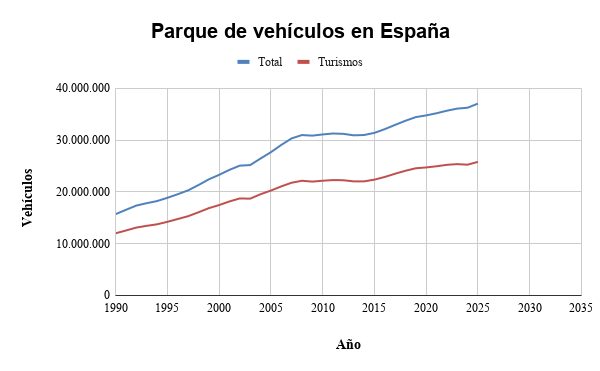
\includegraphics[width=0.8\textwidth]{images/Parque_movil_espana}
  \caption{Evolución del parque de vehículos en España 1990--2025. Fuente: DGT~\cite{dgt2025series}.}
  \label{fig:parque-movil-espana}
\end{figure}

Ese volumen tiene un coste real en tiempo. El informe anual de movilidad urbana de \textit{INRIX}~\cite{inrix2022} estima que los conductores españoles dedican una media de 24 horas al año exclusivamente a buscar aparcamiento. En las grandes ciudades la cifra sube: Madrid, Barcelona y Valencia se sitúan entre las 20 capitales europeas con mayor tiempo de búsqueda. Por ejemplo, en Madrid, los conductores tardan entre 20 y 40 minutos de media en encontrar aparcamiento en zonas céntricas~\cite{parkiduo2025madrid} haciendo que el tiempo en atasco sea de media unas 64 horas.

El aparcamiento regulado en calle y los garajes comerciales reflejan esa presión. En Santa Cruz de Tenerife, el nuevo sistema de zonas azul y verde previsto para 2026~\cite{diariodeavisos2026tarifas} fija tarifas de 1 a 2~€/hora para no residentes en zona azul; los residentes pagarán menos de 1~€/hora o una cuota anual de unos 60~€ en zona verde. En Madrid, el aparcamiento regulado de zona A (SER) alcanza 2,55~€/hora, pero un garaje comercial de centro puede superar los 4,50~€/hora o los 36~€ por 24 horas~\cite{cope2026parking}. En Barcelona, los garajes de máxima demanda superan los 5~€/hora, con jornadas completas en torno a los 30~€~\cite{cope2026parking}.

\begin{table}[H]
  \centering
  \caption{Comparativa de tarifas de aparcamiento regulado por ciudad y zona.}
  \label{tab:tarifas-regulado}
  \begin{tabularx}{\textwidth}{X X c X}
    \toprule
    \textbf{Ciudad}        & \textbf{Zona}       & \textbf{Tarifa (€/hora)} & \textbf{Fuente}       \\
    \midrule
    Santa Cruz de Tenerife & Zona azul (no res.) & 1,00--2,00               & Ayto. Santa Cruz 2026 \\
    Santa Cruz de Tenerife & Zona verde (res.)   & <1,00 / 60\,€/año        & Ayto. Santa Cruz 2026 \\
    Madrid                 & Zona A (SER)        & 2,55                     & EMT / Ayto. Madrid    \\
    Madrid                 & Zona B (SER)        & 1,75                     & EMT / Ayto. Madrid    \\
    Barcelona              & Zona 1 (àrea verda) & 2,75                     & BSM / Ajto. Barcelona \\
    Barcelona              & Zona 2              & 1,40                     & BSM / Ajto. Barcelona \\
    \bottomrule
  \end{tabularx}
\end{table}

\subsection{El mercado en Canarias y el área metropolitana de Tenerife}

Canarias presenta una situación particular. La insularidad limita las alternativas de transporte público y convierte al vehículo privado en la opción dominante para la mayoría de desplazamientos. El Instituto Canario de Estadística~\cite{istac2024} registra en Tenerife una tasa de 870 vehículos por cada 1.000 habitantes en 2025~\cite{eldia2025motoriz} como se puede ver en la \autoref{fig:parque-movil-canarias} siendo esta la más alta del archipiélago, con una edad media del parque superior a los 27~años y más del 13\% de los vehículos superando los 30~años de antigüedad.

La presión sobre el aparcamiento en Santa Cruz de Tenerife y San Cristóbal de La Laguna se explica por la combinación de tres factores: alta densidad residencial en el casco histórico, escasa oferta de aparcamientos públicos subterráneos y concentración de actividad comercial y universitaria. Solo la Universidad de La Laguna, con más de 20.000 estudiantes matriculados, genera una demanda diaria de aparcamiento que actualmente no puede ser absorbida.

A ello se añade la presión normativa ya que la \textit{Ley 7/2021}\footnote{\textbf{Ley 7/2021}: establece la obligatoriedad de las ZBE con carácter vinculante. Santa Cruz de Tenerife (aprox. 210.000 hab.) y San Cristóbal de La Laguna (aprox. 160.000 hab.) quedan dentro de su ámbito de aplicación. La restricción de acceso vehicular no elimina la necesidad de aparcar: la desplaza hacia la periferia, donde la oferta de plazas privadas infrautilizadas es mayor.}, de cambio climático y transición energética~\cite{ley72021}, obliga a los municipios de más de 50.000 habitantes a implantar las ZBE antes del 1 de enero de 2023. Aunque esto se ha ido posponiendo y se prevé que se acabe instaurando en la capital tinerfeña a principios de verano de 2026 haciendo mucho más complicado el acceso al centro urbano de los vehículos antiguos ya mencionados, lo que a su vez incrementa la demanda de aparcamiento en las zonas periféricas.

\begin{figure}[htbp]
  \centering
  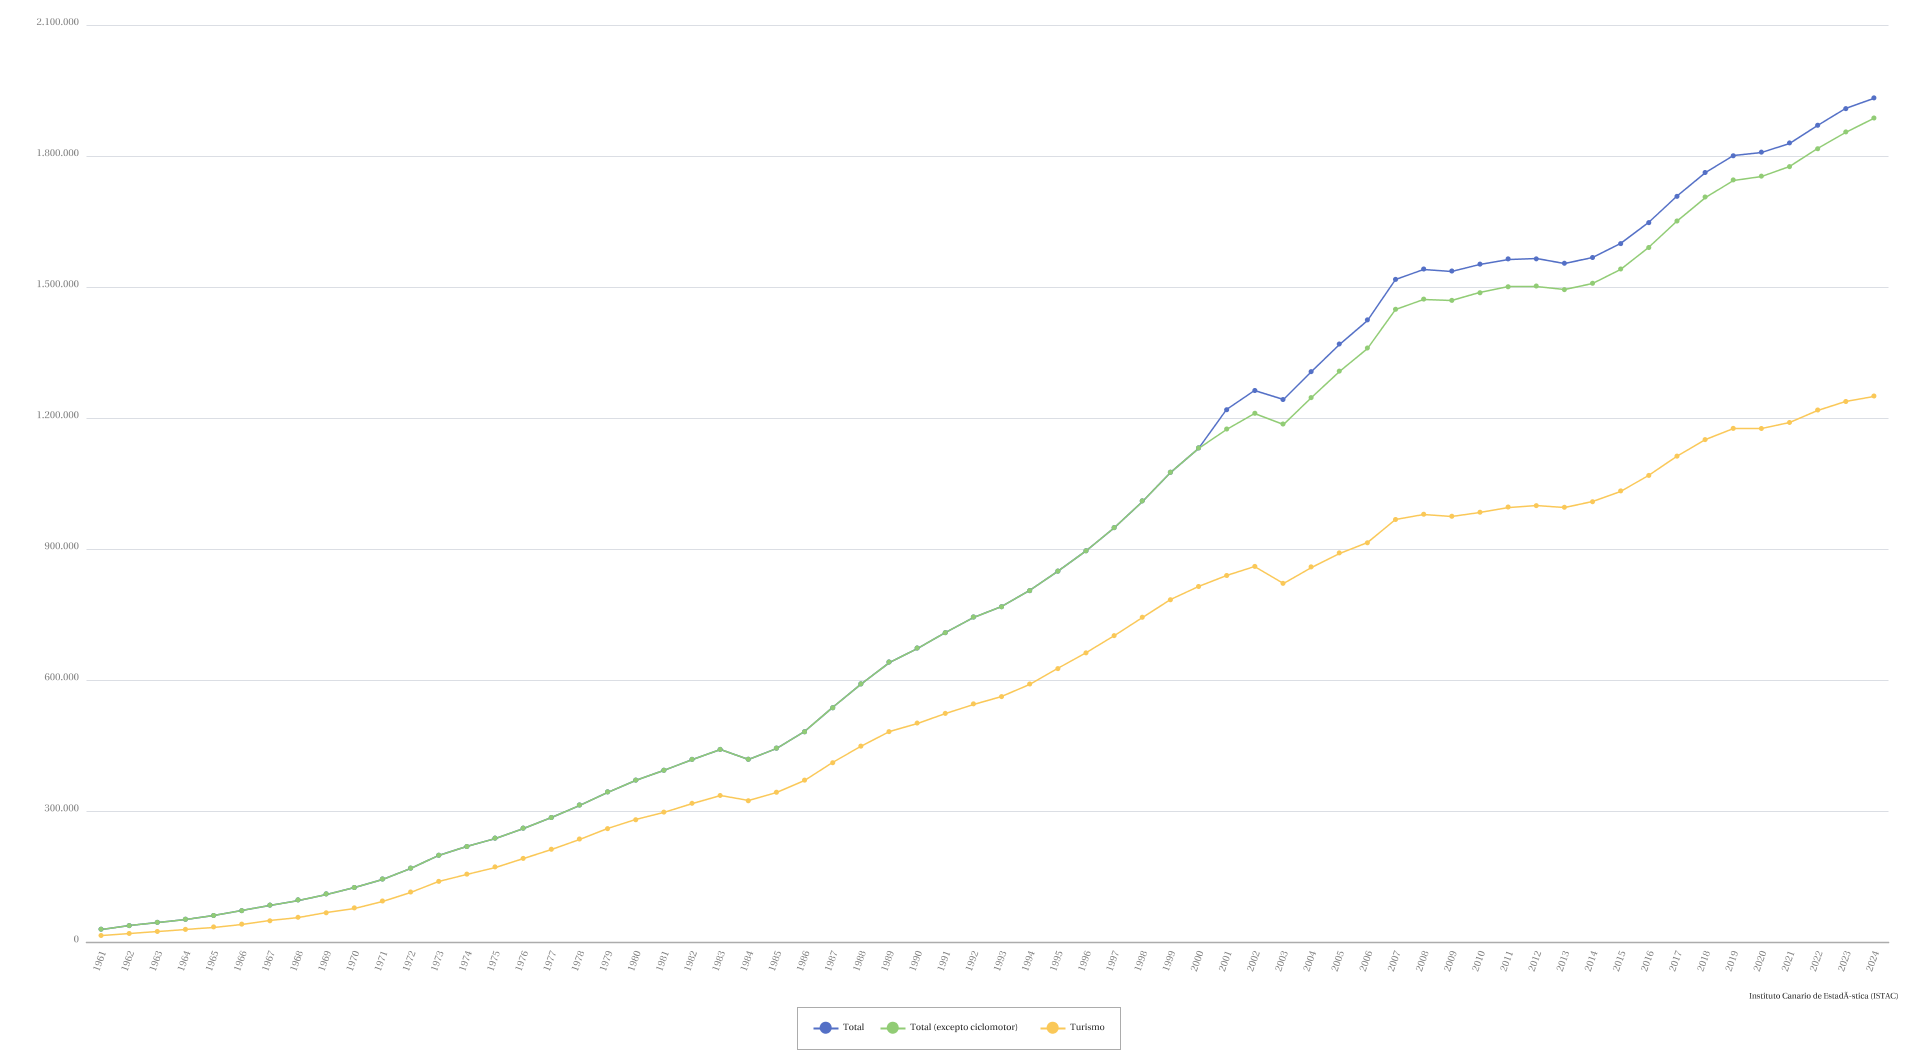
\includegraphics[width=0.9\textwidth]{images/parque_movil_canarias}
  \caption{Evolución anual del parque de vehículos en Canarias (datos desde 1961). Fuente: ISTAC~\cite{istac2024}.}
  \label{fig:parque-movil-canarias}
\end{figure}

\subsection{La Zona de Bajas Emisiones de Santa Cruz de Tenerife}
\label{sec:zbe-sct}

El 13 de abril de 2026, el Ayuntamiento de Santa Cruz de Tenerife aprobó el borrador definitivo de la Ordenanza de Movilidad Sostenible que establece la ZBE municipal~\cite{ayto2026zbe}. La zona abarca 778.244~m\textsuperscript{2} del casco histórico y el distrito Centro, delimitada por la calle Méndez Núñez, la Rambla de Santa Cruz, la avenida de Anaga y el barranco de Santos.

Las restricciones operan de lunes a sábado, de 07:00 a 20:00~horas. Se vetan los vehículos sin etiqueta ambiental DGT: turismos de gasolina matriculados antes de 2001 y diésel anteriores a 2006. La ordenanza prevé 18~meses de carencia para el registro de vehículos y no aplica sanciones efectivas (200~€) hasta 2029.

La normativa contempla una excepción relevante para Parky. Los vehículos con reserva activa en un aparcamiento privado dentro del perímetro quedan exentos de las restricciones ordinarias de acceso. Esta exención convierte a la plataforma en un habilitador de entrada legal al centro urbano, a la vez que redirige la demanda de estacionamiento hacia plazas privadas perimetrales.

\subsection{Disponibilidad y precios en el modelo P2P}

El alquiler de plazas de garaje en Santa Cruz de Tenerife oscila entre 50 y 150~€/mes según ubicación, con la mayor concentración de oferta en el tramo de 60--100~€~\cite{idealista2026garajes} frente a los 7--15~€/día de un parking comercial de rotación. Incluso la tarifa mensual más alta de alquiler resulta competitiva para un conductor que necesita aparcar a diario.

Para el propietario, la relación es igualmente favorable. Una plaza que genera 80~€/mes suma 960~€ anuales por un activo que de otro modo permanece vacío. En mercados donde el modelo P2P ya funciona a escala, JustPark~\cite{justpark2026earnings} documenta entre 500 y 3.000 libras anuales por espacio publicado según la ubicación, lo que da una referencia del potencial del modelo.

La restricción principal del modelo P2P no es de precio, sino de oferta organizada. \textbf{No existe en Canarias ninguna plataforma que agregue esas plazas dispersas, las haga visibles en un mapa y gestione la reserva y el acceso de forma automática.} Esa ausencia define el nicho que Parky busca cubrir.

\section{Objetivos}
\label{sec:objetivos}

\subsection*{Objetivo general}

El objetivo general es diseñar y desarrollar un prototipo funcional de \textit{marketplace P2P} para el alquiler de plazas de aparcamiento privadas en el área metropolitana de Tenerife, que conecte a propietarios de garajes infrautilizados con conductores que necesitan estacionar, y que resuelva de forma integrada la gestión de reservas, el acceso físico al garaje y el flujo de pagos entre particulares.

\subsection*{Objetivos específicos}

\begin{enumerate}

  \item[\textbf{OE1.}] Implementar un sistema de autenticación y control de acceso basado en roles (RBAC)\footnote{\textbf{RBAC} (\textit{Role-Based Access Control}): modelo que asigna permisos a los usuarios según el rol que desempeñan, sin conceder permisos individuales a cada cuenta.} que diferencie la lógica de permisos entre arrendatarios, propietarios y administradores, con soporte para inicio de sesión mediante proveedores externos (OAuth)\footnote{\textbf{OAuth} (\textit{Open Authorization}): protocolo que permite a aplicaciones externas acceder a recursos de un usuario mediante tokens de acceso, sin que este comparta sus credenciales directamente.}.

  \item[\textbf{OE2.}] Construir una \textit{Single Page Application}\footnote{\textbf{SPA} (\textit{Single Page Application}): aplicación web que carga un único documento HTML y actualiza su contenido dinámicamente mediante JavaScript, sin recargar la página desde el servidor.} con enfoque \textit{mobile-first} (ya que la mayoría de reservas se realizan desde móviles) que integre búsqueda sobre mapa interactivo, filtros bidireccionales en tiempo real y geocodificación para el registro de nuevas plazas de aparcamiento.

  \item[\textbf{OE3.}] Garantizar el aislamiento de datos entre usuarios mediante políticas de seguridad (\textit{Row Level Security}, RLS)\footnote{\textbf{RLS} (\textit{Row Level Security}): mecanismo de PostgreSQL que restringe el acceso a filas de una tabla según políticas definidas en el esquema, sin depender de filtros en la capa de aplicación.} aplicadas directamente en el esquema relacional de PostgreSQL.

  \item[\textbf{OE4.}] Prevenir solapamientos en reservas concurrentes mediante \textit{triggers} y procedimientos almacenados en PL/pgSQL, con validación de disponibilidad de plaza ejecutada íntegramente en base de datos, independiente del cliente que origine la petición.

  \item[\textbf{OE5.}] Implementar el flujo de \textit{checkout}, separando automáticamente la tarifa base del arrendador, la comisión de la plataforma y el IGIC del 7\,\% correspondiente a la jurisdicción canaria, y liquidando los pagos directamente a la cuenta bancaria del propietario.

  \item[\textbf{OE6.}] Implementar los estados de reservas mediante rutinas programadas en base a la hora y día actuales, el módulo SmartAccess de apertura remota de garajes con trazabilidad de accesos, y un sistema de valoraciones bidireccionales entre arrendatario y propietario que incentive la confianza en el intercambio entre particulares.

  \item[\textbf{OE7.}] Desplegar la aplicación como cliente web y como aplicación Android nativa desde una base de código TypeScript compartida, utilizando Capacitor\footnote{\textbf{Capacitor}: herramienta de Ionic que empaqueta una aplicación web en un contenedor nativo iOS/Android, dando acceso a las APIs del dispositivo con un único código fuente.} como puente entre la capa web y el sistema operativo móvil.


\end{enumerate}
